\documentclass[aspectratio=169]{beamer}

% Theme and colors
\usetheme{Madrid}
\usecolortheme{seahorse}
\setbeamertemplate{navigation symbols}{}
\setbeamertemplate{footline}{
  \hfill\insertframenumber/\inserttotalframenumber\hspace*{2mm}\vspace{2mm}
}

% Packages
\usepackage{amsmath,amssymb}
\usepackage{graphicx}
\usepackage{tikz}
\usepackage{booktabs}
\usepackage{xcolor}
\usepackage{pgfplots}
\usepackage{animate}
\pgfplotsset{compat=1.17}
\usetikzlibrary{shapes.geometric, arrows.meta, positioning, calc, shadows, fit, backgrounds, overlay-beamer-styles}

% Custom colors
\definecolor{cluster0}{RGB}{255,127,14}
\definecolor{cluster1}{RGB}{31,119,180}
\definecolor{smls_blue}{RGB}{44,62,80}
\definecolor{smls_green}{RGB}{39,174,96}
\definecolor{smls_red}{RGB}{192,57,43}

% Title info
\title[SMLS Model]{\textbf{A Stochastic Machine Learning Surrogate Model\\for Comprehensive Replacement of Spray Submodels}}
\subtitle{ILASS-Americas 36th Annual Conference}
\author[Mishra et al.]{Rohit Mishra\inst{1} \and Advaith Sankaranarayanan\inst{2} \and Kapil Sachdev\inst{3}}
\institute[TAMU]{
    \inst{1}Dept. of Mechanical Engineering, Texas A\&M University\\
    \inst{2}Robbinsville High School, NJ\\
    \inst{3}Dept. of Petroleum Engineering, University of Alaska Fairbanks
}
\date{May 11--14, 2026}

\begin{document}

% =============================================================================
% SLIDE 1: TITLE / OVERVIEW
% =============================================================================
\begin{frame}
\titlepage
\end{frame}

% =============================================================================
% SLIDE 2: OVERVIEW / OUTLINE
% =============================================================================
\begin{frame}{Overview}
\begin{columns}[T]
\begin{column}{0.55\textwidth}
\textbf{Goal:} Replace expensive Lagrangian spray submodels with a trained ML surrogate

\vspace{0.3cm}
\begin{itemize}[<+->]
    \item Physics-informed unsupervised clustering (GMM)
    \item Cluster-specialized expert neural networks
    \item Supervised gating network for routing
    \item Near-perfect ensemble R$^2$ = \textbf{0.9974}
\end{itemize}
\end{column}
\begin{column}{0.42\textwidth}
\pause
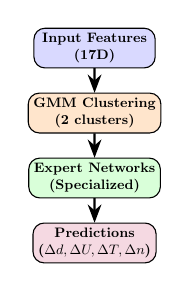
\begin{tikzpicture}[scale=0.55, transform shape,
    box/.style={rectangle, draw, rounded corners, minimum width=2.8cm, minimum height=0.7cm, font=\small\bfseries, align=center}]
    \node[box, fill=blue!15] (input) at (0,4) {Input Features\\(17D)};
    \node[box, fill=orange!20] (gmm) at (0,2.5) {GMM Clustering\\(2 clusters)};
    \node[box, fill=green!15] (experts) at (0,1) {Expert Networks\\(Specialized)};
    \node[box, fill=purple!15] (output) at (0,-0.5) {Predictions\\($\Delta d, \Delta U, \Delta T, \Delta n$)};
    \draw[-Stealth, thick] (input) -- (gmm);
    \draw[-Stealth, thick] (gmm) -- (experts);
    \draw[-Stealth, thick] (experts) -- (output);
\end{tikzpicture}
\end{column}
\end{columns}
\end{frame}

% =============================================================================
% TRANSITION: INTRODUCTION
% =============================================================================
\begin{frame}{}
\vfill
\begin{center}
{\Huge\textbf{Introduction}}
\end{center}
\vfill
\end{frame}

% =============================================================================
% SLIDE 3: INTRODUCTION
% =============================================================================
\begin{frame}{Introduction: Lagrangian-Eulerian Spray Simulation}
\begin{itemize}[<+->]
    \item Modern spray simulations use \textbf{Lagrangian particle tracking} within Eulerian flow fields
    \item Each parcel requires iterative evaluation of:
    \begin{itemize}
        \item Drag correlations
        \item Evaporation models  
        \item Breakup (KH-RT) models
        \item Heat transfer models
    \end{itemize}
    \item Computational cost $\propto$ number of parcels $\times$ submodel evaluations
    \item 4,000--25,000 active parcels per timestep $\Rightarrow$ \textbf{millions of submodel calls}
\end{itemize}

\vspace{0.2cm}
\pause
\begin{alertblock}{Key Insight}
Particle dynamics exhibits \textit{learnable patterns} from state variables $\Rightarrow$ ML surrogates can replace expensive submodels
\end{alertblock}
\end{frame}

% =============================================================================
% TRANSITION: MOTIVATION
% =============================================================================
\begin{frame}{}
\vfill
\begin{center}
{\Huge\textbf{Motivation}}
\end{center}
\vfill
\end{frame}

% =============================================================================
% SLIDE 4: MOTIVATION
% =============================================================================
\begin{frame}{Motivation: Why ML Surrogates?}
\begin{columns}[T]
\begin{column}{0.48\textwidth}
\textbf{\color{smls_red}Challenges in Current Approach:}
\begin{itemize}[<+->]
    \item Empirical models tuned to specific fuels/domains
    \item Poor generalization across injection conditions
    \item Non-tractable for industrial multi-spray systems
    \item Features span vastly different scales:\\
    velocity $\sim 1$ m/s vs. diameter $\sim 10^{-5}$ m
\end{itemize}
\end{column}
\begin{column}{0.48\textwidth}
\pause
\textbf{\color{smls_green}Data-Driven Solution (SMLS):}
\begin{itemize}[<+->]
    \item Standard Unsupervised Clustering (SUC)
    \item More interpretable than generic MoE
    \item Physics-informed clustering via non-dimensional numbers
    \item Trained on high-fidelity 3D CFD data
    \item Single property cannot determine evolution $\Rightarrow$ \textbf{unsupervised multi-feature clustering}
\end{itemize}
\end{column}
\end{columns}
\end{frame}

% =============================================================================
% TRANSITION: SIMULATION SETUP
% =============================================================================
\begin{frame}{}
\vfill
\begin{center}
{\Huge\textbf{Simulation Setup}}
\end{center}
\vfill
\end{frame}

% =============================================================================
% SLIDE 5: SIMULATION SETUP
% =============================================================================
\begin{frame}{Simulation Setup: CFD Spray Dataset}
\begin{columns}[T]
\begin{column}{0.45\textwidth}
\textbf{OpenFOAM 3D Spray Simulation:}
\begin{itemize}
    \item<2-> Water spray: $\rho=988$ kg/m$^3$, $\sigma=0.0675$ N/m
    \item<3-> Hot ambient: 800 K, 5 MPa
    \item<4-> 200 timesteps, 241,000 unique parcels
    \item<5-> Submodels: breakup + evaporation + drag + heat transfer
\end{itemize}

\vspace{0.2cm}
\onslide<6->{
\textbf{Dataset Statistics:}
\footnotesize
\begin{itemize}
    \item Total pairs: 2,423,037
    \item Train/Val/Test: 80/10/10\%
    \item Input: 17D (10 Lag. + 7 Eul.)
    \item Output: 6 targets
\end{itemize}
}
\end{column}
\begin{column}{0.53\textwidth}
\onslide<2->{
\begin{center}
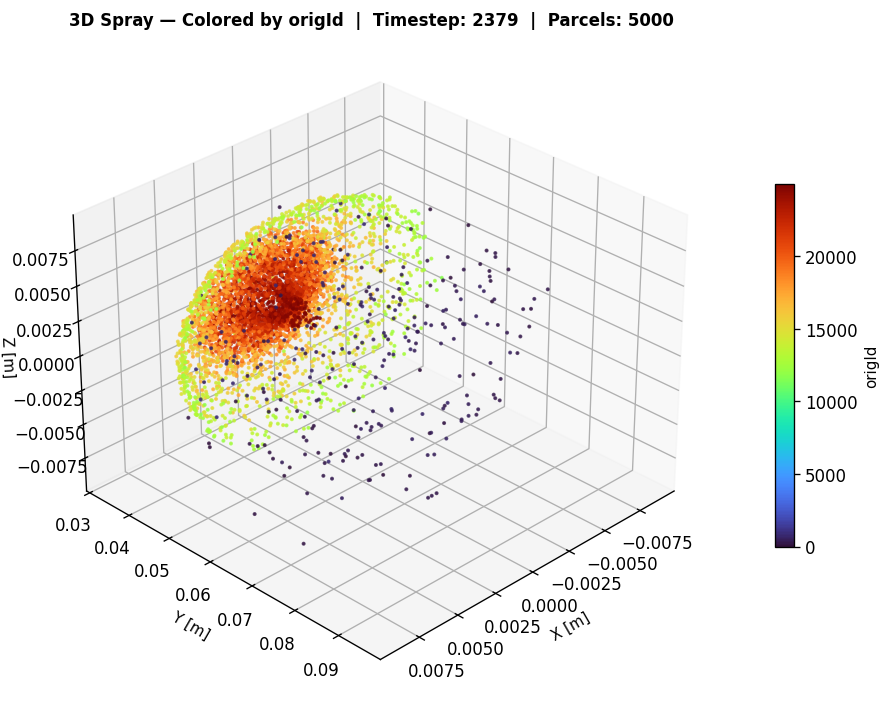
\includegraphics[width=\textwidth]{spray_frames/frame_010.png}
\end{center}
\vspace{-0.2cm}
\begin{center}
\tiny\textit{3D spray colored by origId (25,000 parcels, mid-timestep)}
\end{center}
}
\end{column}
\end{columns}
\end{frame}

% =============================================================================
% SLIDE 5b: SPRAY VISUALIZATIONS (1/2)
% =============================================================================
\begin{frame}{Spray Visualization: Particle Properties}
\begin{columns}[T]
\begin{column}{0.48\textwidth}
\begin{center}

\includegraphics[width=\textwidth]{spray_frames_nParticle/frame_010.png}

\vspace{0.1cm}
\small\textbf{nParticle} — Number of particles per parcel
\end{center}
\end{column}
\begin{column}{0.48\textwidth}
\begin{center}

\includegraphics[width=\textwidth]{spray_frames_diameter/frame_010.png}

\vspace{0.1cm}
\small\textbf{Diameter} — Droplet size evolution
\end{center}
\end{column}
\end{columns}
\end{frame}

% =============================================================================
% SLIDE 5c: SPRAY VISUALIZATIONS (2/2)
% =============================================================================
\begin{frame}{Spray Visualization: Flow Properties}
\begin{columns}[T]
\begin{column}{0.48\textwidth}
\begin{center}

\includegraphics[width=\textwidth]{spray_frames_velocity_mag/frame_010.png}

\vspace{0.1cm}
\small\textbf{Velocity Magnitude} — Momentum exchange with gas
\end{center}
\end{column}
\begin{column}{0.48\textwidth}
\begin{center}

\includegraphics[width=\textwidth]{spray_frames_temperature/frame_010.png}

\vspace{0.1cm}
\small\textbf{Temperature} — Heating from 323K ambient (800K)
\end{center}
\end{column}
\end{columns}
\end{frame}

% =============================================================================
% TRANSITION: NN ARCHITECTURE
% =============================================================================
\begin{frame}{}
\vfill
\begin{center}
{\Huge\textbf{Neural Network Architecture}}
\end{center}
\vfill
\end{frame}

% =============================================================================
% SLIDE 6: NN ARCHITECTURE
% =============================================================================
\begin{frame}{SMLS Architecture: Standard Unsupervised Clustering (SUC)}
\begin{center}
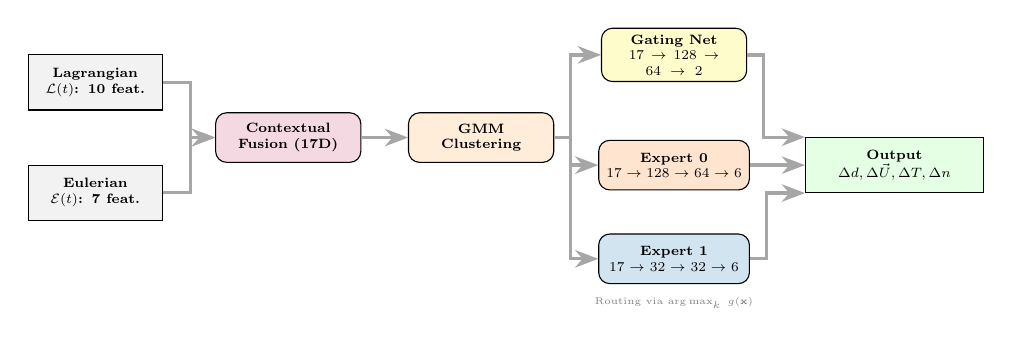
\begin{tikzpicture}[scale=0.7, transform shape,
    node distance=0.8cm,
    data/.style={rectangle, draw, fill=gray!10, text width=2.2cm, text centered, minimum height=1cm, font=\scriptsize\bfseries},
    layer/.style={rectangle, draw, fill=blue!15, text width=2.4cm, text centered, rounded corners, minimum height=0.9cm, font=\scriptsize\bfseries},
    expert/.style={rectangle, draw, rounded corners, text width=2.5cm, text centered, minimum height=0.9cm, font=\scriptsize\bfseries},
    output/.style={rectangle, draw, fill=green!10, text width=3cm, text centered, minimum height=1cm, font=\scriptsize\bfseries},
    arrow/.style={-Stealth, line width=1.2pt, gray!70}
]
    % Inputs
    \node[data] (lag) at (0,2) {Lagrangian\\$\mathcal{L}(t)$: 10 feat.};
    \node[data] (eul) at (0,0) {Eulerian\\$\mathcal{E}(t)$: 7 feat.};
    
    % Fusion
    \node[layer, fill=purple!15] (fuse) at (3.5,1) {Contextual\\Fusion (17D)};
    
    % GMM
    \node[layer, fill=orange!15] (gmm) at (7,1) {GMM\\Clustering};
    
    % Gating
    \node[layer, fill=yellow!20] (gate) at (10.5,2.5) {Gating Net\\$17\to128\to64\to2$};
    
    % Experts
    \node[expert, fill=cluster0!20] (exp0) at (10.5,0.5) {Expert 0\\$17\to128\to64\to6$};
    \node[expert, fill=cluster1!20] (exp1) at (10.5,-1.2) {Expert 1\\$17\to32\to32\to6$};
    
    % Output
    \node[output] (out) at (14.5,0.5) {Output\\$\Delta d, \Delta\vec{U}, \Delta T, \Delta n$};
    
    % Arrows
    \draw[arrow] (lag.east) -- ++(0.5,0) |- (fuse.west);
    \draw[arrow] (eul.east) -- ++(0.5,0) |- (fuse.west);
    \draw[arrow] (fuse) -- (gmm);
    \draw[arrow] (gmm.east) -- ++(0.3,0) |- (gate.west);
    \draw[arrow] (gmm.east) -- ++(0.3,0) |- (exp0.west);
    \draw[arrow] (gmm.east) -- ++(0.3,0) |- (exp1.west);
    \draw[arrow] (gate.east) -- ++(0.3,0) |- (out.north west);
    \draw[arrow] (exp0.east) -- (out.west);
    \draw[arrow] (exp1.east) -- ++(0.3,0) |- (out.south west);
    
    % Labels
    \node[font=\tiny, color=gray] at (10.5, -2.0) {Routing via $\arg\max_k\; g(\mathbf{x})$};
\end{tikzpicture}
\end{center}

\vspace{-0.2cm}
\pause
\begin{equation*}
\hat{\Delta Y}_{\text{ensemble}} = \sum_{k=0}^{1} \mathbb{1}\left[k = \arg\max_k\; g(\mathbf{x}; \boldsymbol{\theta}_{gate})\right] \cdot f_k(\mathbf{x}; \boldsymbol{\theta}_k)
\end{equation*}
\end{frame}

% =============================================================================
% TRANSITION: GMM CLUSTERING
% =============================================================================
\begin{frame}{}
\vfill
\begin{center}
{\Huge\textbf{GMM Clustering}}
\end{center}
\vfill
\end{frame}

% =============================================================================
% SLIDE 7: GMM MODEL
% =============================================================================
\begin{frame}{GMM Clustering: Physics-Informed Regime Discovery}
\textbf{Feature space for GMM:}
\begin{equation*}
\mathcal{G} = \{We,\; Re,\; \Delta d,\; \Delta T,\; \Delta n_{Particle},\; \Delta U_{rel,mag}\}
\end{equation*}

\pause
\vspace{0.1cm}
\begin{columns}[T]
\begin{column}{0.48\textwidth}
\textbf{\color{cluster0}Cluster 0: Small/Volatile (13.7\%)}
\begin{itemize}[<+->]
    \item 265,715 training samples
    \item High We $>$ 5 (strong breakup)
    \item High evaporation rates
    \item $d \sim 10$--$50\;\mu$m
    \item Rapid diameter/temperature changes
\end{itemize}
\end{column}
\begin{column}{0.48\textwidth}
\pause
\textbf{\color{cluster1}Cluster 1: Large/Inert (86.3\%)}
\begin{itemize}[<+->]
    \item 1,674,017 training samples
    \item Low We $<$ 5 (no breakup)
    \item Slow evaporation
    \item $d > 50$--$100\;\mu$m
    \item Stable, deterministic evolution
\end{itemize}
\end{column}
\end{columns}

\vspace{0.3cm}
\pause
\begin{block}{Key Non-Dimensional Numbers}
\vspace{-0.2cm}
\begin{columns}
\begin{column}{0.32\textwidth}
\begin{equation*}
Re_p = \frac{\rho_g |\vec{U}_{rel}| d}{\mu_g}
\end{equation*}
\end{column}
\begin{column}{0.32\textwidth}
\begin{equation*}
We = \frac{\rho_g |\vec{U}_{rel}|^2 d}{\sigma}
\end{equation*}
\end{column}
\begin{column}{0.32\textwidth}
\begin{equation*}
U_{rel} = |\vec{U}_p - \vec{U}_g|
\end{equation*}
\end{column}
\end{columns}
\end{block}
\end{frame}

% =============================================================================
% SLIDE 8a: GMM RESULTS (1/2)
% =============================================================================
\begin{frame}{GMM Results: Non-Dimensional \& Size Distributions}
\begin{columns}[T]
\begin{column}{0.48\textwidth}
\begin{center}
\textbf{Weber \& Reynolds Number}
\vspace{0.1cm}

\includegraphics[width=\textwidth]{../archive/paper/cluster_distributions_We_Re.png}
\end{center}
\end{column}
\begin{column}{0.48\textwidth}
\begin{center}
\textbf{Diameter Change ($\Delta d$)}
\vspace{0.1cm}

\includegraphics[width=\textwidth]{../archive/paper/cluster_distributions_diameter_changes.png}
\end{center}
\end{column}
\end{columns}
\end{frame}

% =============================================================================
% SLIDE 8b: GMM RESULTS (2/2)
% =============================================================================
\begin{frame}{GMM Results: Thermal \& Velocity Distributions}
\begin{columns}[T]
\begin{column}{0.48\textwidth}
\begin{center}
\textbf{Temperature \& Particle Change}
\vspace{0.1cm}

\includegraphics[width=\textwidth]{../archive/paper/cluster_distributions_temperature_particle_change.png}
\end{center}
\end{column}
\begin{column}{0.48\textwidth}
\begin{center}
\textbf{Relative Velocity ($U_{rel}$)}
\vspace{0.1cm}

\includegraphics[width=\textwidth]{../archive/paper/cluster_distributions_urel_mag.png}
\end{center}
\end{column}
\end{columns}
\end{frame}

% =============================================================================
% TRANSITION: SUPERVISED LEARNING
% =============================================================================
\begin{frame}{}
\vfill
\begin{center}
{\Huge\textbf{Supervised Learning}}
\end{center}
\vfill
\end{frame}

% =============================================================================
% SLIDE 9: SUPERVISED LEARNING WITH GATING NETWORK
% =============================================================================
\begin{frame}{Supervised Learning: Gating + Expert Networks}
\textbf{Three-Phase Training Pipeline:}

\vspace{0.2cm}
\begin{columns}[T]
\begin{column}{0.55\textwidth}
\begin{enumerate}
    \item<2-> \textbf{Phase 1: Gating Network}
    \begin{itemize}
        \item $17 \to 128 \to 64 \to 2$ (softmax)
        \item Cross-entropy loss on GMM labels
        \item \textbf{Accuracy: 99.42\%} (10 epochs)
    \end{itemize}
    
    \vspace{0.15cm}
    \item<3-> \textbf{Phase 2: Expert 0} (Small drops)
    \begin{itemize}
        \item $17 \to 128 \to 64 \to 6$
        \item 150 epochs, LR: 5e-5, batch: 64
        \item \textbf{Test loss: 0.0447, R$^2$ = 0.9875}
    \end{itemize}
    
    \vspace{0.15cm}
    \item<4-> \textbf{Phase 3: Expert 1} (Large drops)
    \begin{itemize}
        \item $17 \to 32 \to 32 \to 6$
        \item 15 epochs, LR: 1e-3, batch: 256
        \item \textbf{Test loss: 0.00077, R$^2$ = 0.9990}
    \end{itemize}
\end{enumerate}
\end{column}
\begin{column}{0.42\textwidth}
\onslide<2->{

\includegraphics[width=\textwidth]{../archive/paper/gating_loss_curve.png}
}

\vspace{0.1cm}
\onslide<3->{

\includegraphics[width=0.49\textwidth]{../archive/paper/expert0_loss_curve.png}

\includegraphics[width=0.49\textwidth]{../archive/paper/expert1_loss_curve.png}
}
\end{column}
\end{columns}

\vspace{0.2cm}
\onslide<5->{
\begin{block}{Loss Functions}
\vspace{-0.3cm}
\begin{equation*}
L_{gate} = -\sum_i y_i \log \hat{y}_i \qquad\qquad L_k = \frac{1}{N_k}\sum_{i\in k} \|\Delta\hat{Y}_i - \Delta Y_i\|^2
\end{equation*}
\end{block}
}
\end{frame}

% =============================================================================
% TRANSITION: RESULTS
% =============================================================================
\begin{frame}{}
\vfill
\begin{center}
{\Huge\textbf{Results}}
\end{center}
\vfill
\end{frame}

% =============================================================================
% SLIDE 10: RESULTS & CONCLUSIONS
% =============================================================================
\begin{frame}{Results: Prediction Performance}
\begin{columns}[T]
\begin{column}{0.48\textwidth}
\textbf{Expert 0: Small/Volatile Drops (R$^2$=0.9875)}

\vspace{0.1cm}

\includegraphics[width=\textwidth]{../archive/paper/expert0_predictions.png}
\end{column}
\begin{column}{0.48\textwidth}
\pause
\textbf{Expert 1: Large/Inert Drops (R$^2$=0.9990)}

\vspace{0.1cm}

\includegraphics[width=\textwidth]{../archive/paper/expert1_predictions.png}
\end{column}
\end{columns}

\vspace{0.1cm}
\pause
\begin{center}
\begin{alertblock}{Ensemble R$^2$}
\vspace{-0.2cm}
\begin{equation*}
R^2_{\text{ens}} = 0.137\!\times\!0.9875 + 0.863\!\times\!0.9990 = \mathbf{0.9974}
\end{equation*}
\end{alertblock}
\end{center}
\end{frame}

% =============================================================================
% TRANSITION: CONCLUSIONS
% =============================================================================
\begin{frame}{}
\vfill
\begin{center}
{\Huge\textbf{Conclusions}}
\end{center}
\vfill
\end{frame}

% =============================================================================
% SLIDE 11: CONCLUSION
% =============================================================================
\begin{frame}{Conclusions}
\begin{itemize}[<+->]
    \item Developed \textbf{SMLS}: a stochastic ML surrogate replacing Lagrangian spray submodels
    \item Physics-informed GMM clustering discovers \textbf{two distinct regimes}:
    \begin{itemize}
        \item Cluster 0: Small/volatile drops (high We, rapid breakup/evaporation)
        \item Cluster 1: Large/inert drops (low We, stable, deterministic)
    \end{itemize}
    \item Gating network achieves \textbf{99.42\% accuracy} in cluster routing
    \item Cluster-specialized experts achieve:
    \begin{itemize}
        \item Expert 0 (small drops): R$^2$ = 0.9875
        \item Expert 1 (large drops): R$^2$ = 0.9990
    \end{itemize}
    \item Ensemble model: \textbf{R$^2$ = 0.9974} across all 6 output features
    \item SUC architecture is more interpretable and accurate than monolithic MoE
\end{itemize}
\end{frame}

% =============================================================================
% TRANSITION: FUTURE WORK
% =============================================================================
\begin{frame}{}
\vfill
\begin{center}
{\Huge\textbf{Future Work}}
\end{center}
\vfill
\end{frame}

% =============================================================================
% SLIDE 12: FUTURE WORK
% =============================================================================
\begin{frame}{Future Work}
\begin{columns}[T]
\begin{column}{0.48\textwidth}
\textbf{Model Enhancements:}
\begin{itemize}[<+->]
    \item \textbf{Recursive Unsupervised Clustering}\\Hierarchical regime discovery (primary vs.\ secondary breakup, evaporation vs.\ drag dominated)
    \item \textbf{Physics Loss Augmentation}
    \begin{itemize}
        \item Mass: $L_{mass}$
        \item Momentum: $L_{mom}$
        \item Energy: $L_{energy}$
    \end{itemize}
    \item \textbf{Non-dimensional Abstraction Layer}\\Train on $Re$, $We$, $St$, $Oh$ for generalization across spray configurations
\end{itemize}
\end{column}
\begin{column}{0.48\textwidth}
\pause
\textbf{Integration \& Validation:}
\begin{itemize}[<+->]
    \item \textbf{OpenFOAM Integration}\\Deploy via TensorFlow C API (as in Mishra et al.\ 2022, 2026)
    \item \textbf{Collision Modeling}\\Graph-based approach for inter-parcel interactions
    \item \textbf{Multi-Spray Generalization}\\Train on diverse fuels, injectors, and ambient conditions
    \item \textbf{A-posteriori Validation}\\Full coupled simulation with ML surrogate replacing submodels
\end{itemize}
\end{column}
\end{columns}
\end{frame}

% =============================================================================
% TRANSITION: Q&A
% =============================================================================
\begin{frame}{}
\vfill
\begin{center}
{\Huge\textbf{Questions \& Discussion}}
\end{center}
\vfill
\end{frame}

% =============================================================================
% SLIDE 13: Q&A
% =============================================================================
\begin{frame}{}
\vfill
\begin{center}
{\Huge\textbf{Questions?}}

\vspace{1cm}
{\large Rohit Mishra}\\
{\normalsize rmishra@tamu.edu}

\vspace{0.8cm}
{\footnotesize Code: \texttt{github.com/ctftamu/hybridUnsupervisedClustering}}
\end{center}
\vfill
\end{frame}

\end{document}
